% %%%%%%%%%%%%%%%%%%%%%%%%%% Figure Map_location_Oslofjord %%%%%%%%%%%%%%%%%%%%%%%%%%%%
\begin{figure}[h]
 \setlength{\unitlength}{1.0cm}
 \begin{center}
  \begin{pspicture}(0,0)(15,9)
% Include graphs
   \rput[bl](-0.1,1.0){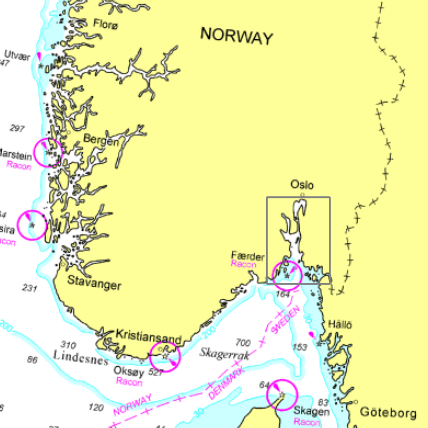
\includegraphics[height=7.3cm]{Map_location_Oslofjord_2}}
   \rput[br](15.0,0.0){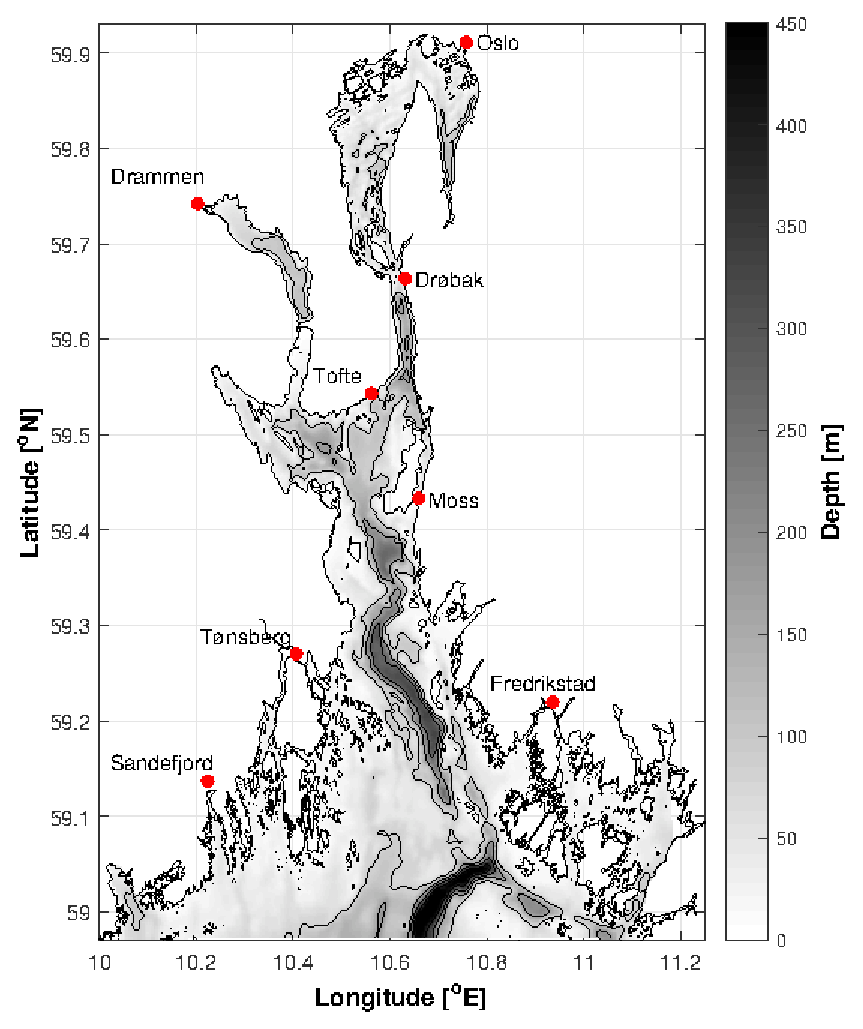
\includegraphics[height=9cm]{dyp_old}}
   \psline[linewidth=0.5mm,linecolor=blue]{->}(13.4,5.3)(11.3,6.3)
   \psline[linewidth=0.2mm](4.45,4.95)(7.5,8.5)
   \psline[linewidth=0.2mm](4.45,3.5)(7.5,1)
  \end{pspicture}
% Figure caption is below the figure
  \caption{\small The topography and irregular coastline of the Oslofjord and its location in Southern Norway. The right-hand gray scale bar indicates depth in meters. The blue arrow points to the location of the fjord's main sill (the {\DR} sill as enlarged in Figure \ref{fig:droebak_sill}) which is only $\sim$ 20 m deep. Note also the $\sim$ 400 m deep basin extending from the Skagerrak towards the Hvaler Archipelago in the southeast, the so called Hvalerdjupet. }
  \label{fig:map_oslofj}       % Give a unique label
 \end{center}
\end{figure}
%
